\chapter{Project Organization}
\label{cha:projectorganization}


This chapter will cover how we organized the entire project. We will uncover the the project timeline in the first section, how roles were distributed among the members in the second section and also the major tools and infrastructure used in the final section of the chapter.
\section{Timeline}
\begin{figure}[!ht]
	\centering
	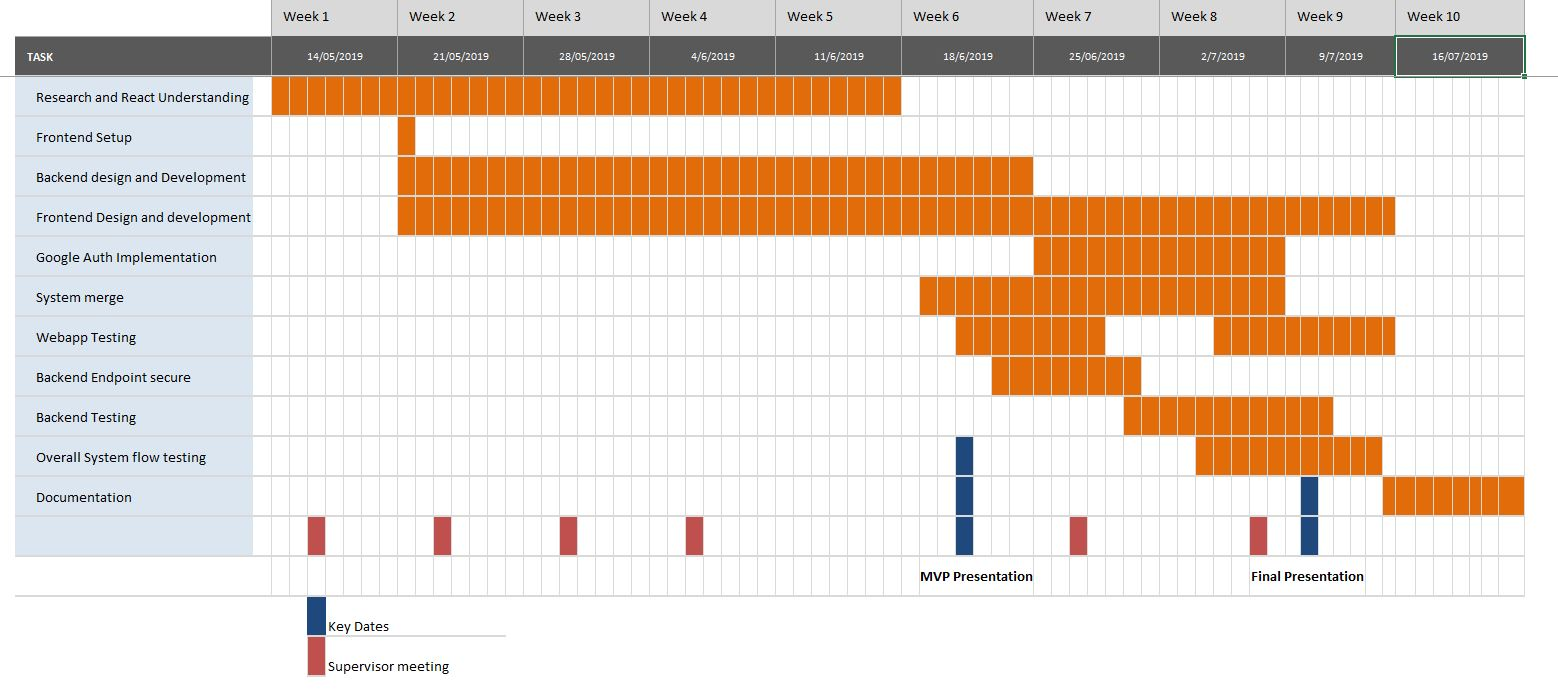
\includegraphics[width=1\textwidth]{images/Timeline.jpg}\\
	\caption{Project Timeline}
	\label{fig:Project Timeline}
\end{figure}

\section{Work Distribution}
\begin{table}[!ht]
\begin{center}
\begin{tabular}{ |l|l|l| } 
 \hline
\textbf{Task} & \textbf{Team Member} \\
 \hline
Customer & Alon \\
 \hline
Company & Kiran  \\
 \hline
 Postman & Anubhav \\
 \hline
 Integration, Routing and Common Web pages & Pradyumna \\
 \hline
 Backend & Haseeb Asif \\
 \hline
  Documentation & All Members \\
 \hline
\end{tabular}
\end{center}
    \caption{ Task Distribution }
\end{table}
To fulfill the requirements of the project in the given time span, we initially divided the task among our team members with five vital tasks and a common task of documenting the code and project as a common task for all the team members as shown in \textbf{table 4.1}.Team member responsible for his/her user space design was responsible to come up with a basic design for the web page and share it among the other team members to be in-sync with the other team members to make sure that the web pages had some consistency through out the project. Git hub was the basic source control used by our team which consisted of the master branch considered to be the actual application and other nodes created by members to work on their relevant tasks.Team member responsible for each user space had the responsibility to develop the complete functionality of the task given to them based on the requirement provided. The team member who was provided with the task of the customer persona was responsible for all customer functionality and so on a similar trend followed for the other major tasks.Integration, routing and common web pages that were common for all personas was a task which included the development of the landing page, user log in,overall routing or navigation inside the application and system integration with back-end. The back-end task which was quite elaborate the team member responsible for the same had to provide an overall database design and implement the same according to the system requirement with appropriate end points being given to the front end developers based on functionality. Documentation of the code and the project was obviously handled by all of the team members to provide inputs on all aspects of their work and the project in general.

Although the tasks are quite strictly divided based on the above task distribution table, we as a team always worked together providing ideas to each other on different tasks to make sure of the overall consistency of the application and also gain collective input and expertise of the entire team where it was necessary.
\section{Tools and Infrastructure}

\begin{itemize}
\item Github - Source control (iosl-dc3, iosl-backend)
\item Trello -Task mgmt (https://trello.com/b/RXwlgcJI/iosl-dc3)
\item Slack - Communication (https://iosltu2019.slack.com)
\item Overleaf- Documentation Collaboration (https://overleaf.com)
\item VS Code - Code editor
\item Azure for Postgres SQL - Database
\end{itemize}
